\documentclass[twoside]{article}

\usepackage[sc]{mathpazo} 
\usepackage[spanish, es-tabla]{babel}
\usepackage[utf8]{inputenc}

\usepackage[hmarginratio=1:1,top=32mm,columnsep=20pt]{geometry} % Document margins
\usepackage{multicol} % Used for the two-column layout of the document
\usepackage[hang, small,labelfont=bf,up,textfont=it,up]{caption} % Custom captions under/above floats in tables or figures
\usepackage{mathtools}
\usepackage{float} % Required for tables and figures in the multi-column environment - [H] needed
\usepackage{hyperref} % For hyperlinks in the PDF with labels

\usepackage{abstract} % Allows abstract customization
\renewcommand{\abstractnamefont}{\normalfont\bfseries} % Set the "Abstract" text to bold
\renewcommand{\abstracttextfont}{\normalfont\small\itshape} % Set the abstract itself to small italic text

\usepackage{titlesec} % Allows customization of titles

\titleformat{\section}[block]{\large\scshape\centering}{\thesection.}{1em}{} % Change the look of the section titles
\titleformat{\subsection}[block]{\large\centering}{\thesubsection.}{1em}{} % Change the look of the section titles

\usepackage{fancyhdr} % Headers and footers
\pagestyle{fancy} % All pages have headers and footers
\fancyhead{} % Blank out the default header
\fancyfoot{} % Blank out the default footer
\fancyhead[C]{Speckle% based on TRACS 
\hspace{4pt} $\bullet$ \hspace{4pt} Diciembre 2018 } % Custom header text
\fancyfoot[RO,LE]{\thepage} % Custom footer text

%----------------------------------------------------------------------------
%	   TITLE SECTION
%----------------------------------------------------------------------------

\title{
	\vspace{-15mm}
	\fontsize{28pt}{10pt}
	\selectfont\textbf{Estudio y Simulación del Efecto de Speckle}% Article title
}

\author{
	\large
	\textsc{Jaime D\'iez Gonz\'alez-Pardo}\\[4mm]
	\fontsize{28pt}{10pt} Universidad de Cantabria \\ % Your institution
	%\thanks{A thank you or further information}\\[2mm] % Your name
	\normalsize Fotónica \\ 
	%\normalsize{Compañeros:} \textsc{NOMBRE COMPANEROS }\\%\normalsize \href{mailto:john@smith.com}{john@smith.com} % Your email address
	%\vspace{5mm}
}

\date{ \today }


%----------------------------------------------------------------------------
%      · DOCUMENT
%----------------------------------------------------------------------------

\begin{document}


	\maketitle % Insert title


	\thispagestyle{fancy} % All pages have headers and footers

%----------------------------------------------------------------------------
%	  ABSTRACT
%----------------------------------------------------------------------------

	\begin{abstract}

		\noindent% Dummy abstract text

			Se ha simulado la obtención de un frente de onda proveniente de una fuente puntual con diferentes fases, para tratar de estudiar el fenómeno de Speckle. Para ello se ha tratado de comprobar la aproximación a la mancha de Airy para diferentes tamaños tanto de la pupila de entrada $D$ como de las zonas con fase constante $r_0$. Se han realizado tres simulaciones para $fase = 0$, $D \approx r_0$ y $D >> r_0$. Para los dos primeros casos sí se ha podido obtener la mancha de Airy, pudiendo observar diferencias entre ambos resultados. Sin embargo en el tercer caso se ha obtenido un patrón de Speckle.

	\end{abstract}

%----------------------------------------------------------------------------
%	  ARTICLE CONTENTS
%----------------------------------------------------------------------------

		\section{Introducción} % Scope of the project = rad effects + minimization
							 
			El estudio de la interferometría Speckle consiste en el análisis del patrón de intensidades producidas por diferentes frentes de onda coherentes pero con diferencias de fases.

			El caso más claro de este fenómeno se encuentra a la hora de tratar de observar las estrellas. Los frentes de onda esféricos emitidos por la estrella y que llegan a la Tierra en forma de frentes de onda planos de igual fase, debido a la gran distancia de la Tierra a la estrella, sufre un cambio de fase diferente en cada uno de sus puntos debido al efecto de la atmósfera en el frente de onda. Esto produce que al tratar de observar la imagen de la estrella, se obtenga el patrón de Speckle. 	

				\begin{figure}[H]
					\centering
					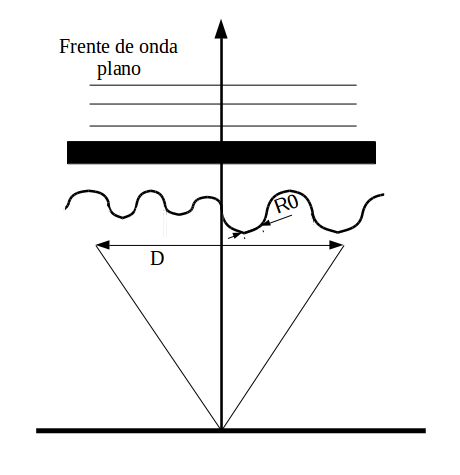
\includegraphics[scale=0.25]{Esquema.png}
					\caption{\label{Img:Esquema}Esquema del sistema simulado para estudiar el efecto Speckle. En la imagen, $D$ corresponde al tamaño de la lente o pupila del telescopio y $R0$ a la aproximación del frente de onda aleatorio en la cuál el frente de onda es constante.}
				\end{figure}

				\newpage

			Para el caso de un foco puntual, si no hubiese cambios en la fase se debería obtener la mancha de Airy. Para el efecto de Speckle se pueden obtener también diferentes aproximaciones a este patrón en función de $D$ y $r_0$:

				\begin{equation}
					\begin{matrix}
						D/r_0 >> 1 & \rightarrow & Imagen \neq Airy
						\\
						D/r_0 << 1 & \rightarrow & Imagen=Airy
					\end{matrix}
					\label{eq:airy}
				\end{equation}

		\section{Desarrollo Experimental}

			El estudio del efecto Speckle producido por diferencias en la fase del frente de onda se ha realizado mediante una simulación a partir del código \cite{Speckle} escrito por el alumno en el lenguaje Python.

			Tanto las pupilas de entrada utilizadas como los frentes de onda se han simulado utilizando el código Espejo.py que permite determinar la forma de la pupila o el valor del frente de onda.

			Para la realización de la simulación se ha partido de una matriz de tamaño $512\times512$ con todos los elementos tomando valor 1. Esta matriz equivaldría a la transformada de Fourier de un único punto, simulando la propagación de una fuente puntual. Para la inroducción de fase aleatoria se muliplica dicha matriz por otra matriz formada por hexágonos. Cada uno de estos hexágonos presentan una fase aleatoria introducida como $tilt$ y $tip$ \ref{eq:Espejo}. De esta forma, se consigue una matriz con diferentes zonas hexagonales con fase constante y distinta para cada uno de los hexágonos. Por último, se multiplica por una matriz compuesta por $1$ en el centro formando un círculo, y el resto ceros. Ésta última matríz equivaldría a la pupila de entrada. El último paso es realizar la transformada de Fourier de la matriz resultante para obtener la imagen final.

			Para el estudio del Speckle, se han modificado lo tamaños tanto de la pupila de la última matriz, cómo de las zonas de fase constante (hexágonos) de la segunda matriz.

		\section{Resultados}

			Durante toda la simulación se ha utilizado un tamaño de imagen  (tamaño de la matriz) cuadrado de $512\times512$

			\subsection{Fuente Puntual}

				Para esta primera parte se ha utilizado un tamaño de pupila grande de diámetro $D = 64$.

				La primera simulación realizada ha sido sin incluir  ningún tipo de fase. En la Figura \ref{Img:airy-normal} se muestran imágenes de la pupila utilizada (gráfica de la izquierda) y de la imagen obtenida (gráfica de la derecha).

					\begin{figure}[H]
						\centering
						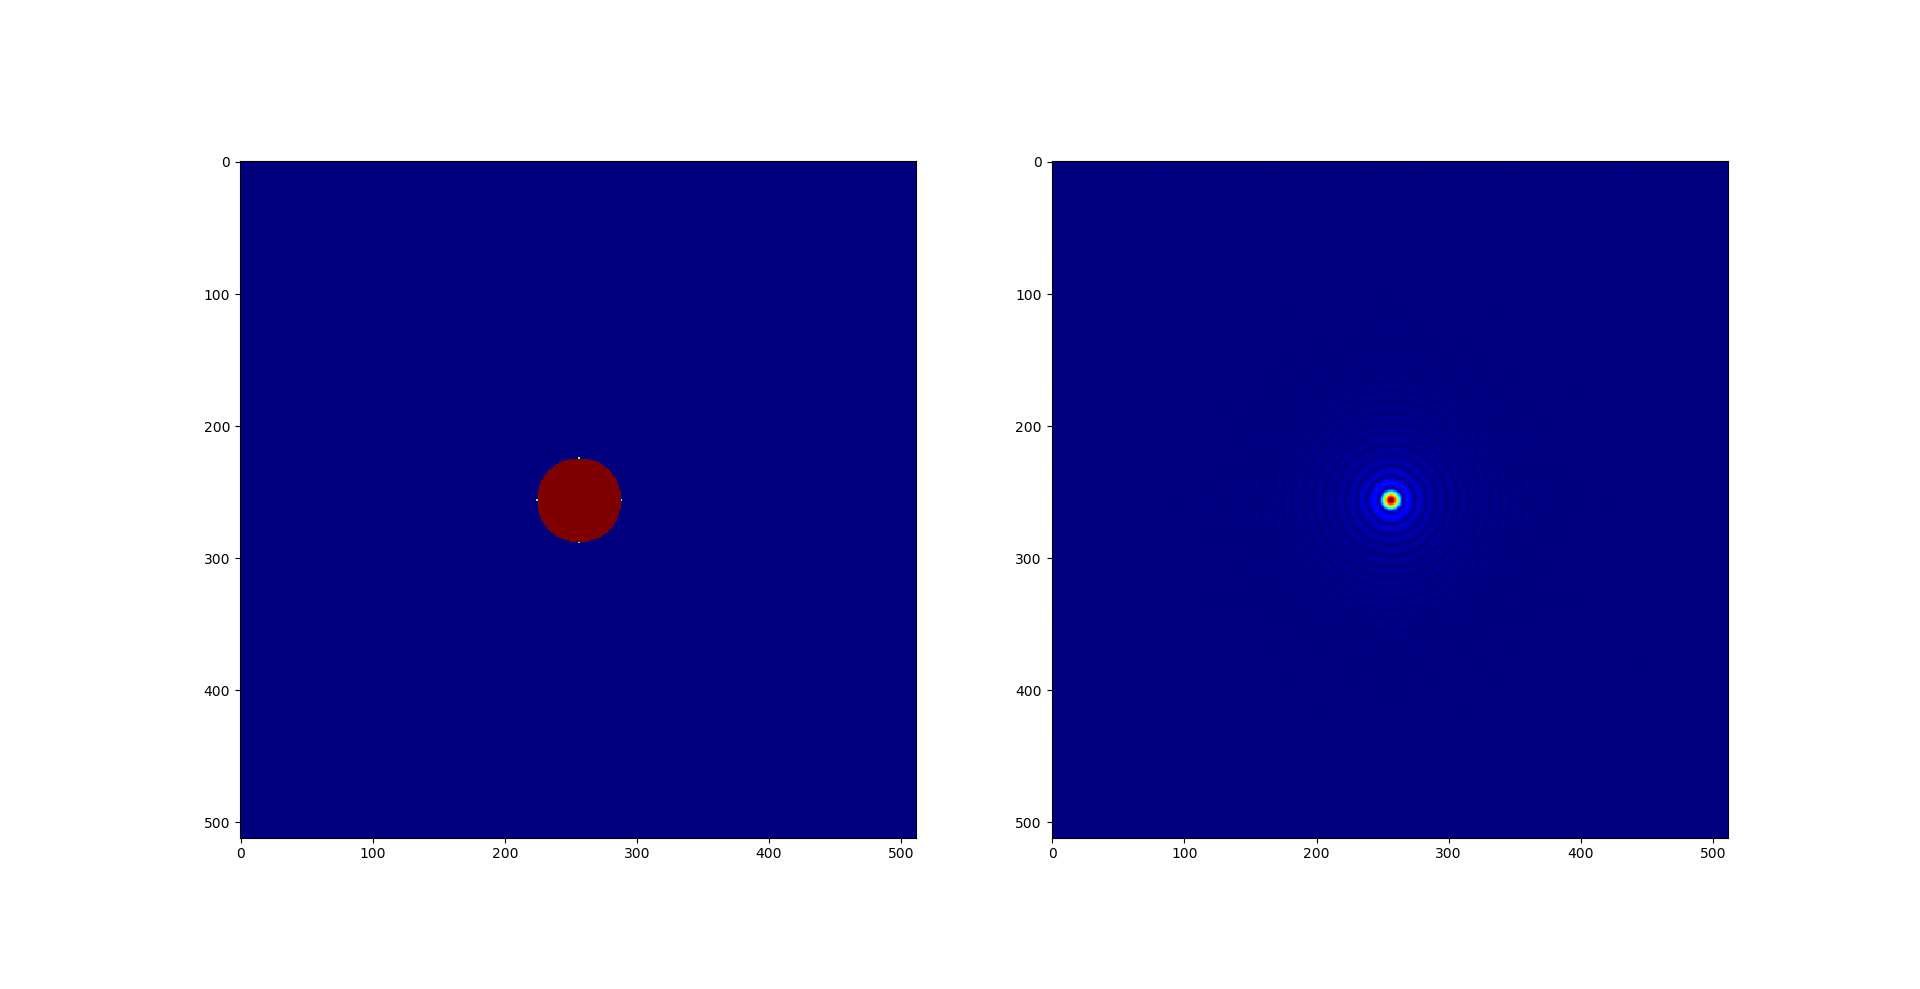
\includegraphics[scale=0.3]{Fig/Hola.png}
						\caption{\label{Img:airy-normal}Pupila de entrada utilizada sin  fase (gráfica de la izquierda) y de la imagen obtenida (gráfica de la derecha).}
					\end{figure}

				En la segunda simulación realizada se han introducido zonas hexagonales con una cierta fase aleatoria para inducir en el frente de onda una fase aleatoria, en este caso el tamaño de las zonas con fase constante (tamaño de los hexagonos) es el mismo que el de la pupila de entrada $r_0 = D = 128$.

				En la Figura \ref{Img:airy-fase} se muestran imágenes de la pupila utilizada (gráfica de la izquierda) y de la imagen obtenida (gráfica de la derecha).

					\begin{figure}[H]
						\centering
						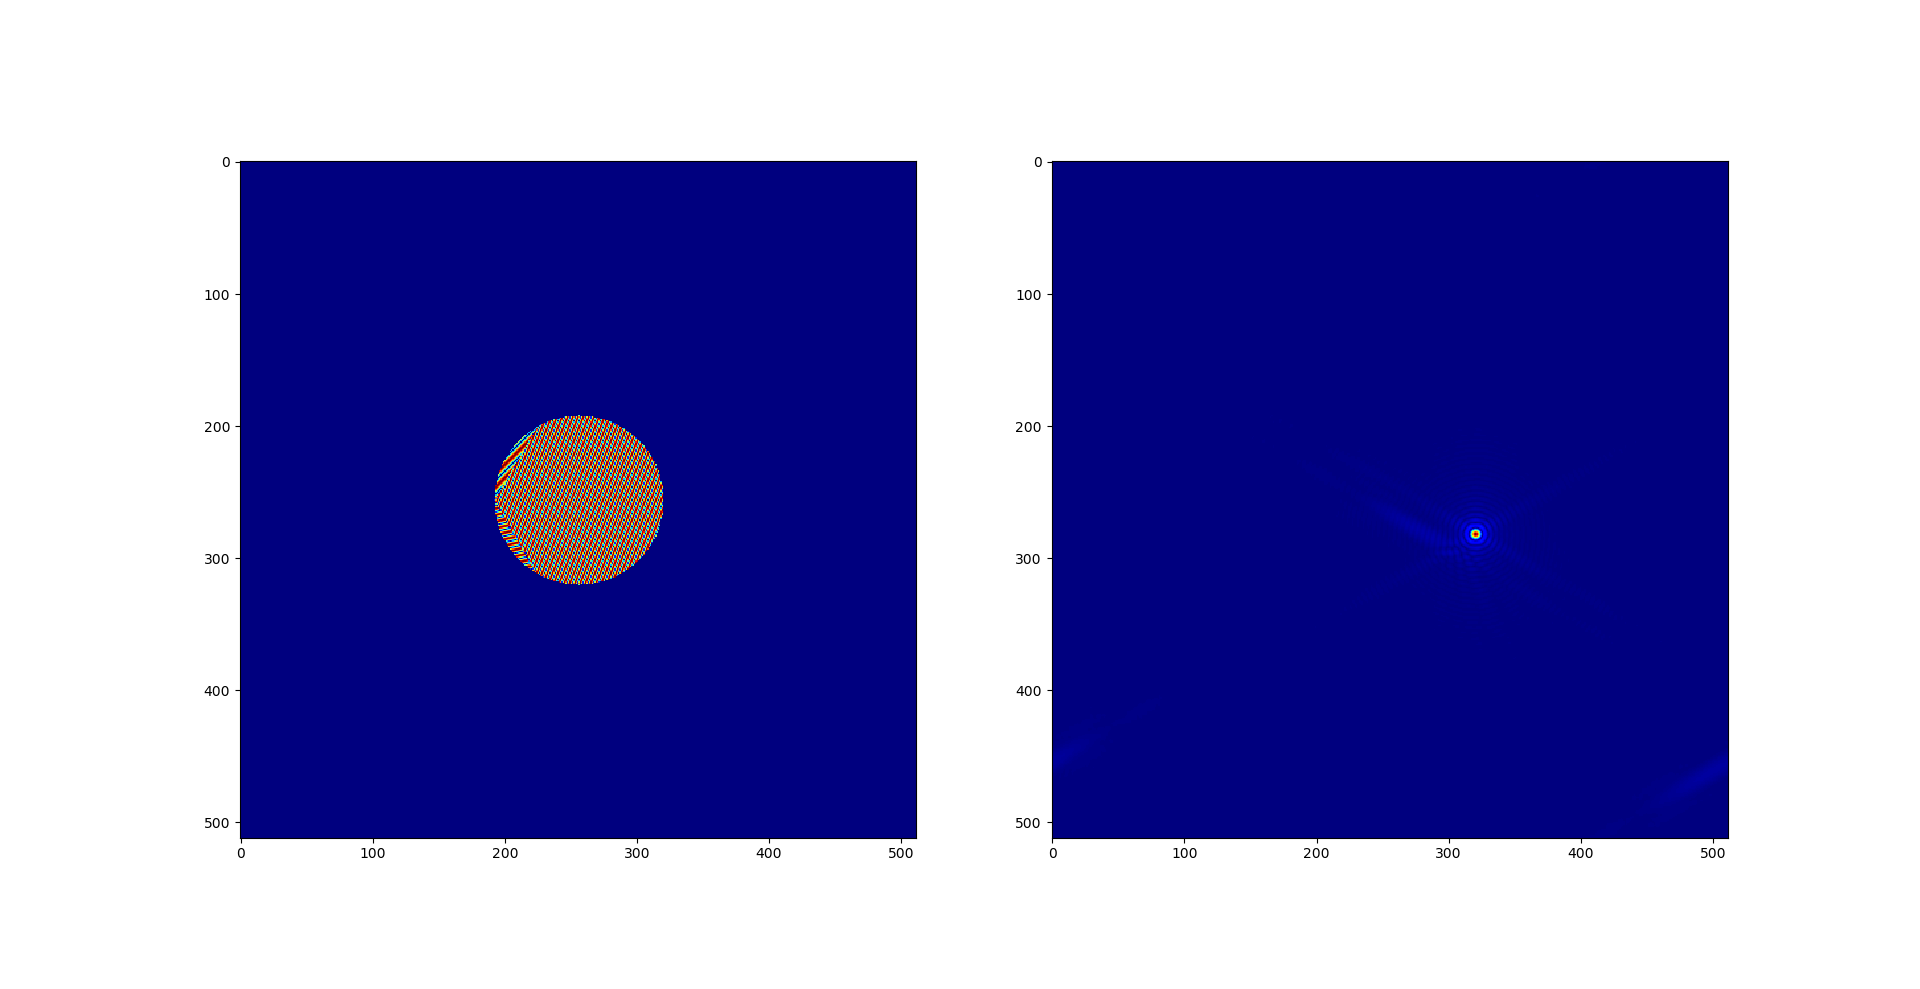
\includegraphics[scale=0.3]{Fig/Airy.png}
						\caption{\label{Img:airy-fase}Pupila de entrada utilizada con zonas con fase aleatoria y contante de tamaño $r_0 = D = 128$ (gráfica de la izquierda) y de la imagen obtenida (gráfica de la derecha).}
					\end{figure}

				Por último, se han utilizado varias zonas hexagonales con fase aleatoria  de tamaño menor a $D$ para formar el frente de onda, en este caso se han utilizado hexagonos de tamaño $r_0 = 16$ y fase aleatoria para cada una de ellas.

				En la Figura \ref{Img:speckle} se muestran imágenes de la pupila de entrada utilizada (gráfica de la izquierda) y de la imagen obtenida (gráfica de la derecha).

					\begin{figure}[H]
						\centering
						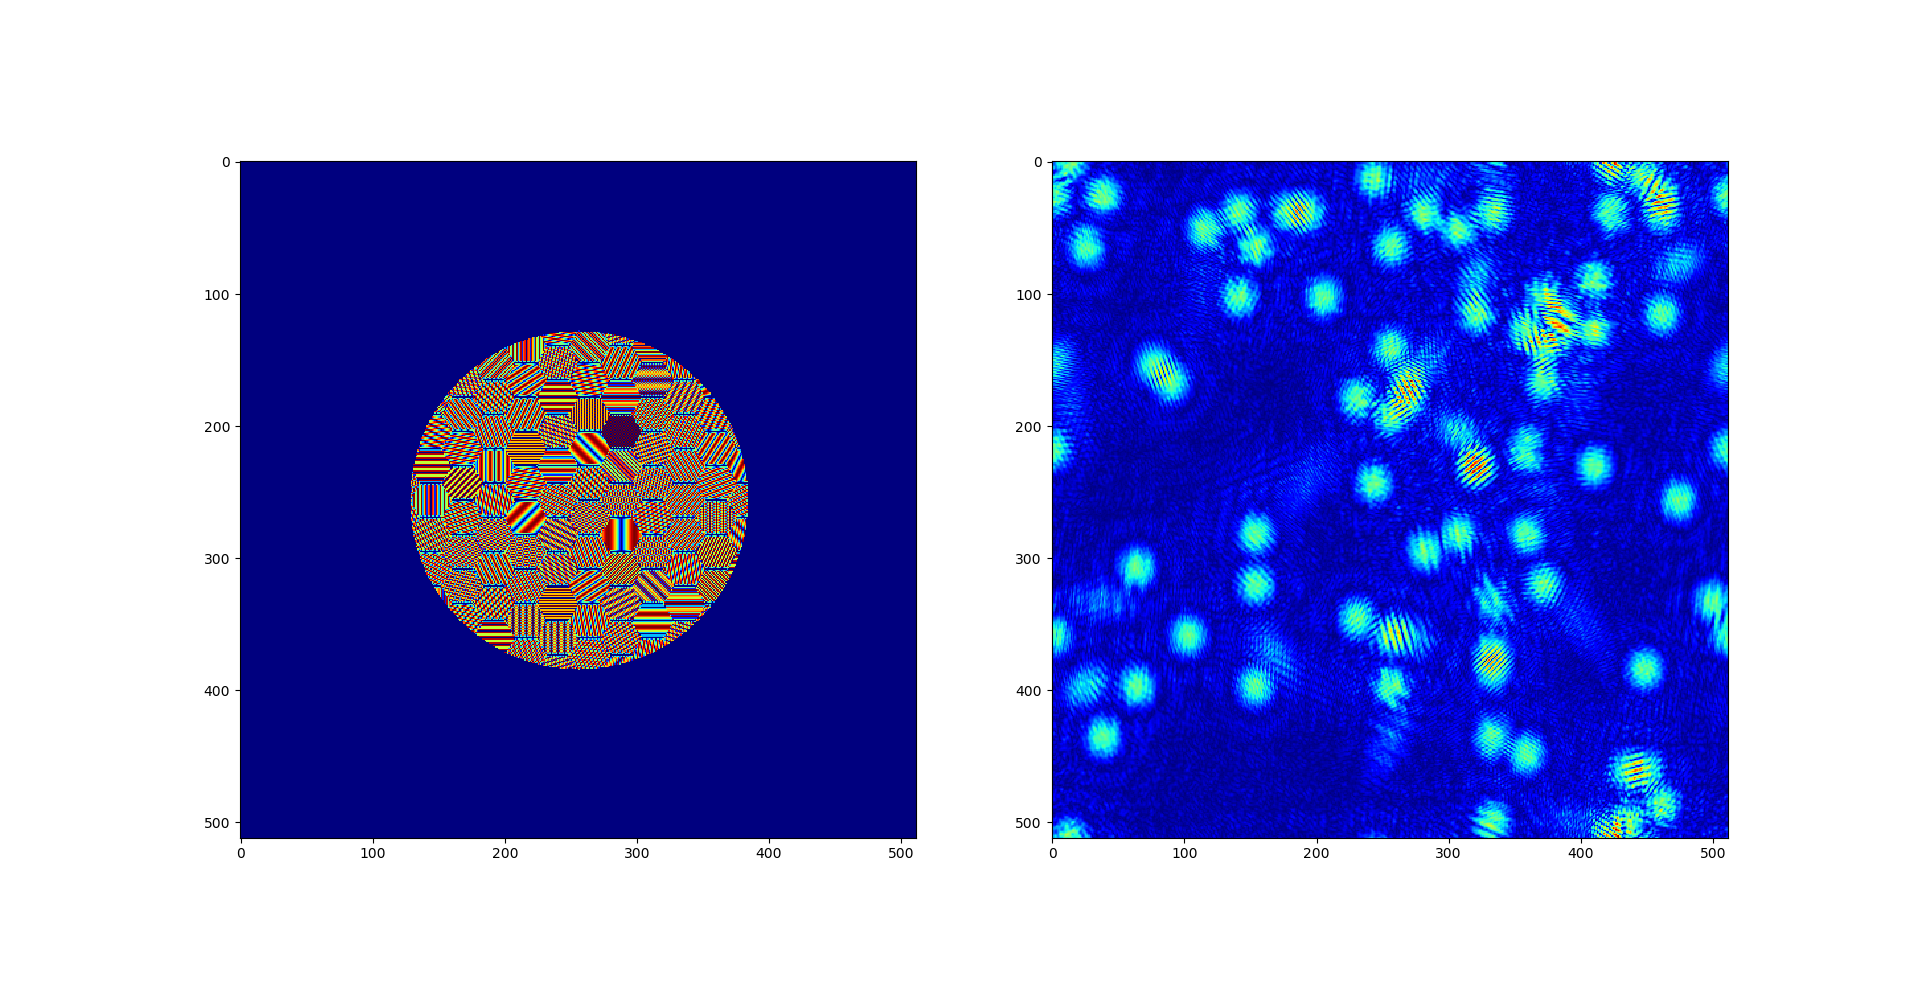
\includegraphics[scale=0.3]{Fig/NoAiry.png}
						\caption{\label{Img:speckle}Pupila de entrada utilizada con zonas con fase aleatoria y constante de tamaño $r_0 = 16$ (gráfica de la izquierda) y de la imagen obtenida (gráfica de la derecha).}
					\end{figure}
		
		\section{Discusión}

			Se han estudiado las intensidades obtenidas a partir de frentes de onda con fases aleatorias tratando de simular los efectos de Speckle.

			En la primera parte se ha estudiado este hecho considerando una fuente puntual, de la cuál se sabe que se ha de obtener la mancha de Airy. En la primera simulación no se ha modificado la fase, obteniendose la mancha de Airy como se puede ver en la figura \ref{Img:airy-normal}.

			Una vez comprobado el resultado de la mancha de Airy se ha introducido zonas con diferentes fases aleatorias. En el primer caso, se han utilizado zonas con $tilt$ y $tip$ constantes de tamaño aproximado al tamaño de la puìla de entrada $D \approx r_0$, obteniendo nuevamente la mancha de Airy pero desplazada del centro y con algunas intensidades diferentes como se puede observar en la figura \ref{Img:airy-fase}. Estas pequeñas diferencias con la mancha de Airy de la primera simulación pueden ser debidas a que la forma de dichas zonas es hexagonal, por lo que en el borde de la pupila se obtendrían zonas con diferente fase (diferente $tilt$ y  $tip$), lo que puede originar dichas diferencias.

			A continuación, se utilizaron zonas con $tilt$ y $tip$ constantes de tamaño mucho menor al tamaño de la pupila $D >> r_0$. Para este caso, se ha podido observar los efectos que produce tener difernecias en la fase de un mismo frente de onda a la hora de obtener su imagen, ya que en la figura \ref{Img:speckle} en la que se muestra el resultado de la simulación, se ha perdido completamente la mancha de Airy.

			Con esta primera parte se ha podido comprobar mediante simulación las aproximaciones de la ecuación \ref{eq:airy}, observando como a medida que $r_0$ disminuye respecto a $D$, se pierde la mancha de Airy.

		\section{Conclusiones}

			Se ha podio estudiar el fenómeno de Speckle pudiendo comprobar mediante una simulación simple las aproximaciones y límites de este fenómeno que se muestran en la ecuación \ref{eq:airy}.


%----------------------------------------------------------------------------
%     APPENDIX
%----------------------------------------------------------------------------

%\newpage

	    \appendix

		    	\section{Obtención de la pupila y el frente de onda}
		    		\label{appen:Espejo}

					Para  $(\sqrt{k^2+j^2}=r_{k,j}) < R$:

						\begin{equation}
							Espejo_{k, j} = 1 \cdot e^{i\cdot crv \cdot r_{k,j}} \cdot e^{i\cdot (tip\cdot r_k + tilt \cdot r_j)}
						\end{equation}
						
					Para $(\sqrt{k^2+j^2}=r_{k,j}) = R$:

						\begin{equation}
							Espejo_{k,j} = 0.5 \cdot e^{i\cdot crv \cdot r_{k,j}} \cdot e^{i\cdot (tip\cdot r_k + tilt \cdot r_j)}
							\label{eq:Espejo}
						\end{equation}	

					Siendo $(k, j)$ las coordenadas $(x, y)$ de la matriz, $r_{k, j}$ el radio de esas coordenadas respecto al centro de la matriz, $R$ el radio del espejo, $crv$ la curvatura, $tip$ la inclinación respecto al eje $X$ y $tilt$ la inclinación respecto al eje $Y$.
	    		
%----------------------------------------------------------------------------
%     BIBLIOGRAPHY
%----------------------------------------------------------------------------

	\bibliographystyle{unsrt}
	\bibliography{biblio}

\end{document}


%----------------------------------------------------------------------------
%            TEMPLATES
%----------------------------------------------------------------------------

%----------------------------------------------------------------------------
%            how to insert an image
%----------------------------------------------------------------------------

%	\begin{figure}[H]
%		\centering
%		\includegraphics[scale= ]{nombre de la imagen.jpg}
%		\caption{\label{Img:widgets}el pie de pagina que le quieras 	poner a la imagen}
%	\end{figure}
 
%----------------------------------------------------------------------------
%            how to insert a table
%----------------------------------------------------------------------------

%	\begin{table}[H]
%		\centering
%		\begin{tabular}{|c|c|c|c|}
%			\hline
%			\centering
%				Altura(h) & Distancia (d) & Elaboracion (e) & Longitud (l) \\
%				($\pm0.5$ mm) & ($\pm0.5$ mm) & ($\pm0.5$ mm) & ($\pm0.5$ mm) \\ \hline
%				 &  &  &  \\ \hline
%				 &  &  &  \\ \hline
%				 &  &  &  \\ \hline
%				 &  &  &  \\ \hline
%				 &  &  &  \\ \hline
%		         &  &  &  \\ \hline
%		\end{tabular}
%		\caption{\label{Tab:widgets}pie de pagina que le quieras poner}
%	\end{table}

%----------------------------------------------------------------------------
%             How to remove the label in equactions
%----------------------------------------------------------------------------

%	\begin{equation*}
%		
%	\end{equation*}

%----------------------------------------------------------------------------
%              How to set bibliography
%----------------------------------------------------------------------------

%\bibliographystyle{unsrt}
%\bibliography{biblio}
%
%Then you have to set a .bib document such as the next template
%
%	@book{nickname,
%	author = {},
%	title = {},
%	edition = {},
%	year = {},
%	volume = {},
%	ISBN = {}
%	}
%
%	@ARTICLE{nickname,
%	author = {},
%	title = {},
%	year = {},
%	volume = {},
%	}


%----------------------------------------------------------------------------
%              END
%----------------------------------------------------------------------------
